\section{Verification and Empirical Evaluation}
\label{sec:verification_evaluation}

This chapter brings together the two forms of evidence on which the present work relies. On the one hand stand the compile-time constraints, unit tests, integration tests, and live-backend checks through which the correctness of the architecture is validated. On the other hand stands the empirical evaluation of the asynchronous layer, whose goal is to show when coroutine-based execution yields a real practical benefit and when its cost remains comparable to or higher than the synchronous alternative.

The important methodological principle is that these two forms of evidence are not treated as interchangeable. Test-based verification answers whether the library is correct with respect to its own contracts and backend limitations. Benchmark evaluation answers a different question: does the asynchronous execution model deliver a measurable benefit under workloads in which the waiting phase dominates local computation. Only the joint presence of both layers makes the architectural claims of the work sufficiently convincing.

\subsection{Verification strategy}

The verification strategy follows the architecture of the library itself. The compile-time layer is checked through concepts, capability restrictions, and typed query-IR construction. The runtime layer is checked through unit tests for rendering, parameter binding, thread safety, migrations, coroutine infrastructure, and asynchronous access. The outermost layer is validated through integration tests against real backends so that mock correctness is not confused with actual driver behaviour.

In the current repository revision, the full automated suite contains 271 tests when executed through \code{ctest}. That number is not in itself a scientific result, but it is important as an indicator that the mechanisms discussed in the preceding chapters are not left at the level of a conceptual scheme. They are covered by systematic checks across layers and backend families.

\begin{table}[H]
\centering
\small
\caption{Principal sources of verification evidence}
\label{tab:evaluation_evidence_matrix}
\begin{tabularx}{\textwidth}{L{3.1cm}L{5.0cm}Z}
\toprule
\textbf{Source} & \textbf{What it validates} & \textbf{Representative artefacts} \\
\midrule
Compile-time constraints and query IR & type correctness of queries, capability-based restriction, and connector contracts & \path{tests/unit/test_query.cpp}, \path{tests/unit/test_postgresql_connector.cpp}, \path{tests/unit/test_mongodb_connector.cpp} \\
Asynchronous infrastructure & \code{Task<T>}, \code{ThreadPool}, \code{IoContext}, \code{async\_db<DB>}, coroutine-aware pooling, and transactions & \path{tests/unit/test_task.cpp}, \path{tests/unit/test_thread_pool.cpp}, \path{tests/unit/test_io_context.cpp}, \path{tests/unit/test_async_connector.cpp} \\
Migrations and thread safety & schema-diff logic, rollback semantics, connection guards, and concurrency safety & \path{tests/unit/test_schema_migration.cpp}, \path{tests/unit/test_thread_safety.cpp} \\
Live backend integration & behaviour across real SQLite, PostgreSQL, MySQL, MongoDB, Redis, Neo4j, and Cassandra environments & \path{tests/integration/test_sqlite.cpp}, \path{tests/integration/test_postgresql_live.cpp}, \path{tests/integration/test_mongodb_live.cpp}, \path{tests/integration/test_redis_live.cpp} \\
Empirical evaluation & throughput under simulated waiting and isolated coroutine-overhead measurements & \path{benchmarks/bench_async.cpp} \\
\bottomrule
\end{tabularx}
\end{table}

Table~\ref{tab:evaluation_evidence_matrix} shows that the evidence base is heterogeneous by necessity. A compile-time ORM library cannot be defended through throughput numbers alone, just as an asynchronous architecture cannot be defended through concept checks alone. Both kinds of evidence are required.

\subsection{Catalogue of unit and integration evidence}

To prevent the verification strategy from remaining at the level of a general framework only, it must also be unfolded as a concrete catalogue of repository artefacts. This is especially important for the present work because the architectural claims are distributed across the entity layer, the query IR, the connector contract, the asynchronous infrastructure, and live-backend checks. The following tables do exactly that: they show where the principal evidence is located in the repository and what role each test group plays.

\begin{table}[H]
\centering
\small
\caption{Principal unit tests for the generic, core, and asynchronous subsystems}
\label{tab:verification_unit_core}
\begin{tabularx}{\textwidth}{L{3.2cm}L{3.8cm}Y}
\toprule
\textbf{File} & \textbf{Subsystem} & \textbf{What it validates} \\
\midrule
\path{test_types.cpp} & basic type aliases & correctness of the public aliases and basic utility dependencies \\
\path{test_property.cpp} & entity property layer & compile-time model of scalar fields and type-trait behaviour \\
\path{test_relationship.cpp} & entity relationship layer & inference logic for relations and storage-strategy behaviour \\
\path{test_query.cpp} & query IR and fluent API & correctness of \code{select}, \code{insert}, \code{update}, \code{deleteq}, and the derived query structures \\
\path{test_schema_migration.cpp} & migration layer & DDL generation, diff logic, and state-machine behaviour \\
\path{test_thread_safety.cpp} & concurrency helpers & behaviour of the connection pool, thread-local access, and transaction-guard mechanism \\
\path{test_task.cpp} & coroutine task abstraction & lifecycle of \code{Task<T>} and basic await/coroutine semantics \\
\path{test_thread_pool.cpp} & worker scheduling & posting, scheduling, and worker-resource coordination \\
\path{test_io_context.cpp} & asynchronous orchestration & event-loop and continuation plumbing for the asynchronous execution layer \\
\path{test_async_connector.cpp} & asynchronous connector facade & bridge logic between \code{async\_db<DB>} and coroutine-aware connector hooks \\
\path{test_wire_protocol.cpp} & experimental execution layer & low-level compile-time and wire-oriented mechanisms \\
\path{test_cpp26_reflection.cpp} & future language integration & early path for reflection-based automation \\
\bottomrule
\end{tabularx}
\end{table}

Table~\ref{tab:verification_unit_core} matters because it shows that the unit layer is not limited to query-parser-like checks. It simultaneously covers the logical model, execution mechanics, migrations, and the coroutine-aware infrastructure on which the asynchronous architecture depends.

\begin{table}[H]
\centering
\small
\caption{Backend-oriented unit tests and their contract focus}
\label{tab:verification_unit_connectors}
\begin{tabularx}{\textwidth}{L{3.4cm}L{3.1cm}Z}
\toprule
\textbf{File} & \textbf{Backend focus} & \textbf{Type of evidence} \\
\midrule
\path{test_postgresql_connector.cpp} & \code{PostgreSQLDB} & \code{is\_connector} compliance, capability asserts, and SQL parameter rendering \\
\path{test_mysql_connector.cpp} & \code{MySQLDB} & joins/transactions contract, dialect-specific rendering, and binding expectations \\
\path{test_mongodb_connector.cpp} & \code{MongoDB} & negative capability validation and BSON-like filter rendering \\
\path{test_redis_connector.cpp} & \code{RedisDB} & absence of joins/transactions/aggregation and key-value command materialisation \\
\path{test_cassandra_connector.cpp} & \code{CassandraDB} & capability restrictions and CQL-rendering correlates \\
\path{test_neo4j_connector.cpp} & \code{Neo4jDB} & transaction capability and graph-oriented query materialisation \\
\bottomrule
\end{tabularx}
\end{table}

These backend-oriented unit tests are critical because they prove not only positive capabilities, but also honestly declared limitations. In a multi-backend library, negative verification --- that a backend \emph{does not} support an operation --- is just as important as positive verification.

\begin{table}[H]
\centering
\small
\caption{Catalogue of integration and live tests}
\label{tab:verification_integration_tests}
\begin{tabularx}{\textwidth}{L{3.2cm}L{3.0cm}Y}
\toprule
\textbf{File} & \textbf{Execution mode} & \textbf{What it demonstrates} \\
\midrule
\path{test_mockdb.cpp} & always-available integration baseline & query composition, parameter binding, prepared queries, and CRUD scenarios without an external backend \\
\path{test_sqlite.cpp} & local integration test & real relational execution path with capability asserts, joins, transactions, and result hydration \\
\path{test_postgresql_live.cpp} & conditional live test & real connection, table lifecycle, and CRUD execution against PostgreSQL \\
\path{test_mysql_live.cpp} & conditional live test & real MySQL driver path, insert/update/delete, and select filtering \\
\path{test_mongodb_live.cpp} & conditional live test & execution of document-oriented scenarios against a live backend \\
\path{test_redis_live.cpp} & conditional live test & key-value and hash-command materialisation in a Redis environment \\
\path{test_cassandra_live.cpp} & conditional live test & wide-column execution and backend-specific CQL scenarios \\
\path{test_neo4j_live.cpp} & conditional live test & graph-query execution through a controlled Docker environment \\
\bottomrule
\end{tabularx}
\end{table}

Table~\ref{tab:verification_integration_tests} shows that the repository-backed evidence is layered. Not all backends have the same operational cost for live verification, but the repository contains a clear strategy for how and when such tests are activated. This matters especially for the thesis because it avoids confusing mock correctness with real driver-backed behaviour.

\subsection{Maturity map according to evidence support}

The capability profile by itself is not sufficient if evidence for actual behaviour is missing. It is therefore useful to examine the backends also as a maturity ladder determined not only by supported operations, but also by available test support. Here maturity means a combination of contract correctness, execution evidence, and operational realism.

\begin{table}[H]
\centering
\small
\caption{Backend maturity map according to the available evidence base}
\label{tab:verification_backend_maturity_map}
\begin{tabularx}{\textwidth}{L{2.4cm}L{2.2cm}L{2.9cm}Y}
\toprule
\textbf{Backend} & \textbf{Maturity level} & \textbf{Principal evidence base} & \textbf{Interpretation} \\
\midrule
\code{MockDB} & level 3 & \path{test_mockdb.cpp} & backend-independent execution baseline for the query contract and prepared-query mechanics \\
SQLite & level 3 to 4 & \path{test_sqlite.cpp} & local real execution path with rich query evidence and capability asserts \\
PostgreSQL & level 3 & \path{test_postgresql_connector.cpp}, \path{test_postgresql_live.cpp} & strong contract plus conditional live-backend verification \\
MySQL & level 3 & \path{test_mysql_connector.cpp}, \path{test_mysql_live.cpp} & real operational path with a relational profile and dialect-specific binding \\
MongoDB & level 3 & \path{test_mongodb_connector.cpp}, \path{test_mongodb_live.cpp} & document-oriented execution evidence without SQL-style capabilities \\
Redis & level 3 & \path{test_redis_connector.cpp}, \path{test_redis_live.cpp} & key-value execution evidence with a restricted but honest contract profile \\
Neo4j & level 3 & \path{test_neo4j_connector.cpp}, \path{test_neo4j_live.cpp} & graph execution path with Docker-gated live verification \\
Cassandra & level 3 & \path{test_cassandra_connector.cpp}, \path{test_cassandra_live.cpp} & wide-column path focused on formal suitability and live coverage \\
\bottomrule
\end{tabularx}
\end{table}

The map in Table~\ref{tab:verification_backend_maturity_map} is important because it prevents an overly binary reading of backend status. A connector is not simply present or absent; it may be contract-correct, execution-validated, partially live-verified, or schema-aware rich. It is exactly this more nuanced reading that makes the verification chapter scientifically stronger and closer to the real state of the repository.

\subsection{Benchmark methodology}

The empirical evaluation is implemented through Google Benchmark~\cite{google_benchmark_user_guide} in \path{benchmarks/bench_async.cpp}. Its purpose is not to simulate the full lifecycle of a concrete database, but to isolate the architectural question of whether coroutine-based execution frees worker threads more effectively than synchronous blocking when a short local CPU phase is separated by a waiting interval.

The benchmark suite is divided into two groups. The first group measures the throughput of whole batches of tasks. The synchronous baseline performs CPU work and then blocks the worker thread for a predefined interval. The asynchronous variant uses the \code{SimulatedAsyncIO} awaitable, which suspends the coroutine, schedules a delayed resumption through a timer queue, and posts the continuation back to \code{ThreadPool}. The second group measures isolated overheads: creation and waiting of \code{Task<int>}, the \code{ThreadPool::post()} round-trip, and nested \code{co\_await} chains.

Methodologically, it is important that the throughput benchmarks use wall-clock time rather than pure CPU time. The reason is explicitly stated in the benchmark source itself: on macOS, calibration by CPU time may behave misleadingly for coroutine scenarios with a waiting phase because a suspended task consumes almost no CPU. The comparison is therefore performed through \code{UseRealTime()} and a fixed number of iterations.

This chapter uses the release-mode results from the local \path{build-rel} build tree. They should not be interpreted as absolute production numbers for all possible machines and drivers. Their role is comparative: all variants are executed on the same machine and with the same parameter grid so that the relative effect of the different execution models can be isolated.

\begin{table}[H]
\centering
\small
\caption{Benchmark families and their purpose}
\label{tab:benchmark_families}
\begin{tabularx}{\textwidth}{L{3.4cm}L{5.2cm}Y}
\toprule
\textbf{Benchmark family} & \textbf{What it measures} & \textbf{Principal parameters} \\
\midrule
\code{BM\_SyncThroughput} & throughput of the blocking baseline, in which the worker thread remains occupied during the waiting phase & number of threads, number of tasks, waiting latency, CPU iterations \\
\code{BM\_AsyncThroughput} & throughput of the coroutine variant with suspend/resume and delayed resumption through a timer queue & number of threads, number of tasks, waiting latency, CPU iterations \\
\code{BM\_AsyncYieldThroughput} & cost of coroutine interleave without artificial waiting latency & number of threads, number of tasks, CPU iterations \\
\code{BM\_TaskCreateAndWait} & minimal cost of creating and completing a trivial task & single coroutine without external scheduling \\
\code{BM\_ThreadPoolPost} & cost of \code{post()} and the promise/future round-trip to a worker thread & size of the thread pool \\
\code{BM\_NestedCoAwait} & overhead of nested \code{co\_await} continuation at different depths & depth of the coroutine chain \\
\bottomrule
\end{tabularx}
\end{table}

\subsection{Principal throughput results}

Table~\ref{tab:throughput_results_release} summarises representative release-mode results for the most informative configurations. It shows direct pairs for which the synchronous and asynchronous variants were measured under the same parameters.

\begin{table}[H]
\centering
\small
\caption{Representative release-mode throughput results for synchronous and asynchronous execution}
\label{tab:throughput_results_release}
\begin{tabularx}{\textwidth}{L{1.3cm}L{1.5cm}L{1.9cm}L{2.4cm}L{2.4cm}L{1.7cm}}
\toprule
\textbf{Threads} & \textbf{Tasks} & \textbf{Waiting latency} & \textbf{Synchronous throughput} & \textbf{Asynchronous throughput} & \textbf{Speedup} \\
\midrule
4 & 100 & 10~$\mu$s & 194.6k ops/s & 658.5k ops/s & 3.38$\times$ \\
4 & 100 & 100~$\mu$s & 29.8k ops/s & 458.2k ops/s & 15.35$\times$ \\
4 & 100 & 1000~$\mu$s & 3.22k ops/s & 75.28k ops/s & 23.36$\times$ \\
4 & 1000 & 100~$\mu$s & 30.08k ops/s & 670.5k ops/s & 22.29$\times$ \\
8 & 100 & 100~$\mu$s & 57.13k ops/s & 258.5k ops/s & 4.53$\times$ \\
\bottomrule
\end{tabularx}
\end{table}

The most important conclusion is that the advantage of the coroutine model grows not when local CPU work grows, but when the waiting phase begins to dominate it. With 4 worker threads and 100 tasks, increasing the waiting latency from 10 to 1000 microseconds ($\mu$s) raises the relative advantage of the asynchronous variant from 3.38$\times$ to 23.36$\times$. This is exactly the expected behaviour: in the synchronous baseline, threads are exhausted by blocking, whereas in the coroutine model they are released for other work.

A second important conclusion is that the effect does not disappear for larger batches. With 4 threads, 1000 tasks, and 100~$\mu$s waiting latency, the asynchronous variant reaches 670.5k operations per second versus 30.08k for the synchronous baseline. This shows that the architectural advantage is not limited to a small demonstration case, but persists when competition for worker resources increases.

\begin{figure}[H]
\centering
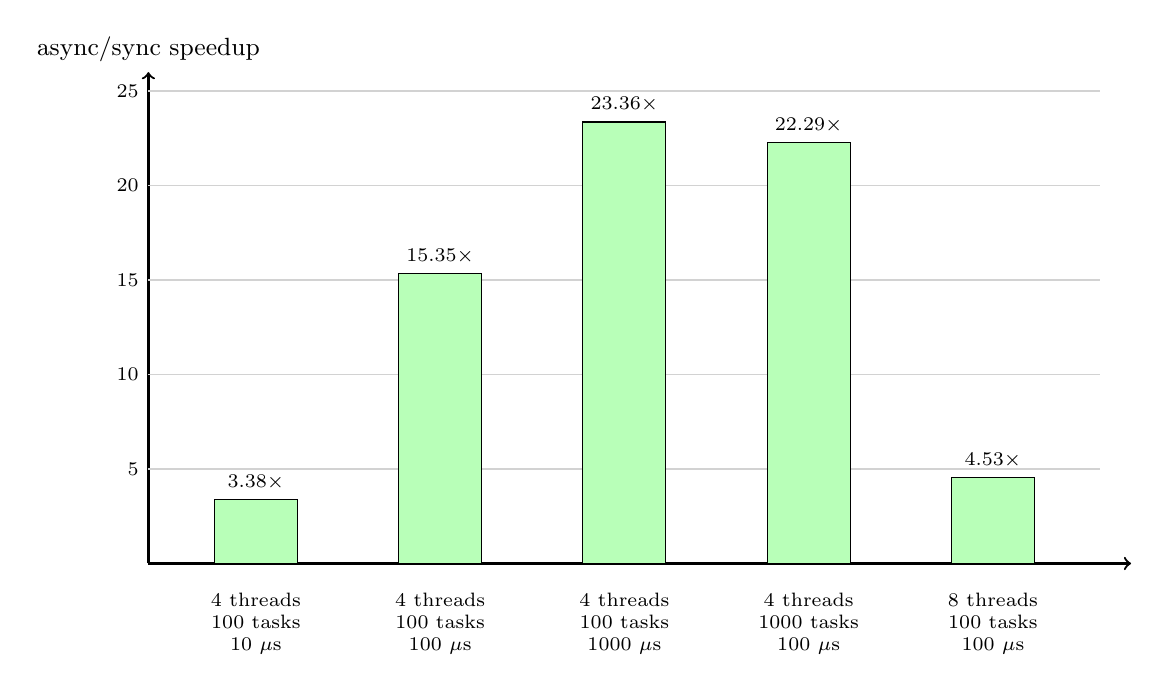
\begin{tikzpicture}[x=1.95cm,y=0.24cm]
    \draw[->, thick] (0,0) -- (0,26) node[above] {\small async/sync speedup};
    \draw[->, thick] (0,0) -- (6.4,0);

    \foreach \y in {5,10,15,20,25}
    {
        \draw[gray!35] (0,\y) -- (6.2,\y);
        \node[left] at (0,\y) {\scriptsize \y};
    }

    \foreach \x/\h/\labeltext/\valuetext in {
        0.7/3.38/{4 threads\\100 tasks\\10~$\mu$s}/3.38,
        1.9/15.35/{4 threads\\100 tasks\\100~$\mu$s}/15.35,
        3.1/23.36/{4 threads\\100 tasks\\1000~$\mu$s}/23.36,
        4.3/22.29/{4 threads\\1000 tasks\\100~$\mu$s}/22.29,
        5.5/4.53/{8 threads\\100 tasks\\100~$\mu$s}/4.53}
    {
        \fill[green!28, draw=black] (\x-0.27,0) rectangle (\x+0.27,\h);
        \node[font=\scriptsize, align=center, above] at (\x,\h) {\valuetext$\times$};
        \node[font=\scriptsize, align=center, below=7pt] at (\x,0) {\labeltext};
    }
\end{tikzpicture}
\caption{Relative speedup of asynchronous throughput over the synchronous baseline in representative I/O-bound configurations}
\label{fig:async_speedup_cases}
\end{figure}

Figure~\ref{fig:async_speedup_cases} visualises the same trend in relative form. Even when the number of worker threads is doubled to 8, the asynchronous variant remains approximately 4.5$\times$ faster at 100~$\mu$s waiting latency. This is a practically relevant result: more threads reduce part of the pressure on the synchronous baseline, but do not eliminate the structural advantage of the suspend/resume execution model.

\subsection{Zero waiting latency (0ns) and coroutine scheduling overhead}

With zero artificial waiting latency, the comparison no longer measures the release of worker threads from I/O waiting and instead begins to expose almost the pure cost of the suspend/resume machinery. For that reason, the most appropriate repository-backed comparison combines \code{BM\_SyncThroughput} with a zero waiting value and \code{BM\_AsyncYieldThroughput}, which replaces the timer-based wait with a single \code{PoolYield} handoff back to \code{ThreadPool}.

\begin{table}[H]
\centering
\small
\caption{Representative release-mode results at zero artificial waiting latency}
\label{tab:zero_latency_yield_results}
\begin{tabularx}{\textwidth}{L{1.4cm}L{1.5cm}L{2.8cm}L{2.9cm}Y}
\toprule
\textbf{Threads} & \textbf{Tasks} & \shortstack{\textbf{Synchronous}\\\textbf{throughput}} & \shortstack{\textbf{Async yield}\\\textbf{throughput}} & \shortstack{\textbf{Ratio}\\\textbf{async/sync}} \\
\midrule
4 & 100 & 841.0k ops/s & 989.4k ops/s & 1.18$\times$ \\
4 & 1000 & 1.232M ops/s & 1.184M ops/s & 0.96$\times$ \\
8 & 100 & 810.9k ops/s & 514.4k ops/s & 0.63$\times$ \\
\bottomrule
\end{tabularx}
\end{table}

\begin{figure}[H]
\centering
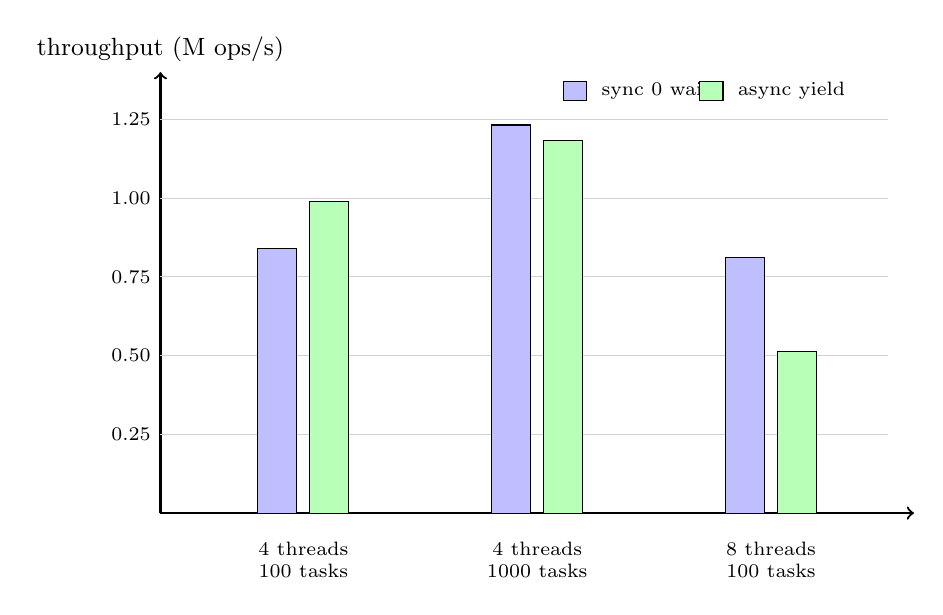
\begin{tikzpicture}[x=1.65cm,y=4.0cm]
    \draw[->, thick] (0,0) -- (0,1.40) node[above] {\small throughput (M ops/s)};
    \draw[->, thick] (0,0) -- (5.8,0);

    \foreach \y/\label in {0.25/0.25,0.50/0.50,0.75/0.75,1.00/1.00,1.25/1.25}
    {
        \draw[gray!35] (0,\y) -- (5.6,\y);
        \node[left] at (0,\y) {\scriptsize \label};
    }

    \fill[blue!25, draw=black] (0.75,0) rectangle (1.05,0.841);
    \fill[green!28, draw=black] (1.15,0) rectangle (1.45,0.989);
    \node[font=\scriptsize, align=center, below=7pt] at (1.10,0) {4 threads\\100 tasks};

    \fill[blue!25, draw=black] (2.55,0) rectangle (2.85,1.232);
    \fill[green!28, draw=black] (2.95,0) rectangle (3.25,1.184);
    \node[font=\scriptsize, align=center, below=7pt] at (2.90,0) {4 threads\\1000 tasks};

    \fill[blue!25, draw=black] (4.35,0) rectangle (4.65,0.811);
    \fill[green!28, draw=black] (4.75,0) rectangle (5.05,0.514);
    \node[font=\scriptsize, align=center, below=7pt] at (4.70,0) {8 threads\\100 tasks};

    \fill[blue!25, draw=black] (3.10,1.31) rectangle (3.28,1.37);
    \node[font=\scriptsize, anchor=west] at (3.32,1.34) {sync 0 wait};
    \fill[green!28, draw=black] (4.15,1.31) rectangle (4.33,1.37);
    \node[font=\scriptsize, anchor=west] at (4.37,1.34) {async yield};
\end{tikzpicture}
\caption{Throughput comparison at zero artificial waiting latency}
\label{fig:zero_latency_yield_throughput}
\end{figure}

Table~\ref{tab:zero_latency_yield_results} and Figure~\ref{fig:zero_latency_yield_throughput} show that, in the absence of a waiting phase, the coroutine layer no longer receives the structural bonus observed in the I/O-bound regime. With 4 threads and 100 tasks, the yield-only variant is still about 1.18$\times$ faster, but with 4 threads and 1000 tasks it is nearly at parity with the synchronous baseline (0.96$\times$), and with 8 threads and 100 tasks it drops to 0.63$\times$. This is a useful corrective to the strong I/O-bound results: without an external wait, the coroutine machinery does not “create” throughput, but instead adds a small yet measurable scheduling cost that can be compensated only partially.

\subsection{Microbenchmark interpretation of overhead}

The isolated overhead measurements show that the coroutine infrastructure is not itself the dominant cost in the I/O-bound scenarios. In the release build, \code{BM\_TaskCreateAndWait} measures approximately 71.6~ns for creation and completion of a trivial task. \code{BM\_ThreadPoolPost} remains around 5.0~$\mu$s regardless of whether the pool has 1, 2, 4, or 8 worker threads. \code{BM\_NestedCoAwait} reaches about 324~ns at depth 10 and about 2.375~$\mu$s even at depth 100.

These numbers should not be read as a direct promised cost of every real query, but they are important for another reason. They show that the overhead of the coroutine machinery is orders of magnitude smaller than the 100--1000~$\mu$s waiting phases under which asynchronous throughput gains the most. In other words, the observed speedup is not an artefact of the measuring tool, but a consequence of worker threads no longer being locked into blocking waits.

\subsection{Limitations of the empirical evaluation}

The empirical evaluation deliberately uses a simulated waiting phase rather than full end-to-end execution against a concrete network database server. This is a limitation if the goal is to predict absolute throughput for a real PostgreSQL or Cassandra deployment. Yet it is also a methodological advantage if the goal is to isolate the execution model from the effects of the Structured Query Language (SQL) planner, network fluctuations, driver caching, and storage-engine specifics.

The present benchmark results therefore do not prove that “asynchronous is always faster”. They prove a narrower but more scientifically defensible claim: when the architecture operates in an I/O-bound regime and the waiting phase dominates local CPU work, a coroutine-based model allows substantially better utilisation of worker resources than the synchronous baseline. That is precisely the claim that the asynchronous layer of the library must justify.

Combined with the test-based verification, this result closes the two principal questions of the thesis. On the one hand, the library demonstrates a formal and test-supported correctness discipline. On the other hand, the asynchronous execution model demonstrates a measurable and practically relevant benefit in exactly the scenario for which it was designed. In this way the empirical evaluation does not stand apart from the architecture, but confirms its central engineering and scientific meaning.
